%! Author = gramic
%! Date = 08.05.24

% Preamble
\begin{flushleft}
    \section{Monitoring}
    Das Monitoring im \Gls{PRTG} besteht aus zwei Teilen.\\
    Zum einen werden die Standard-Werte wie Ping, CPU Load, Load Average, Disk Free, Traffic und die Uptime:
    \begin{figure}[H]
        \centering
        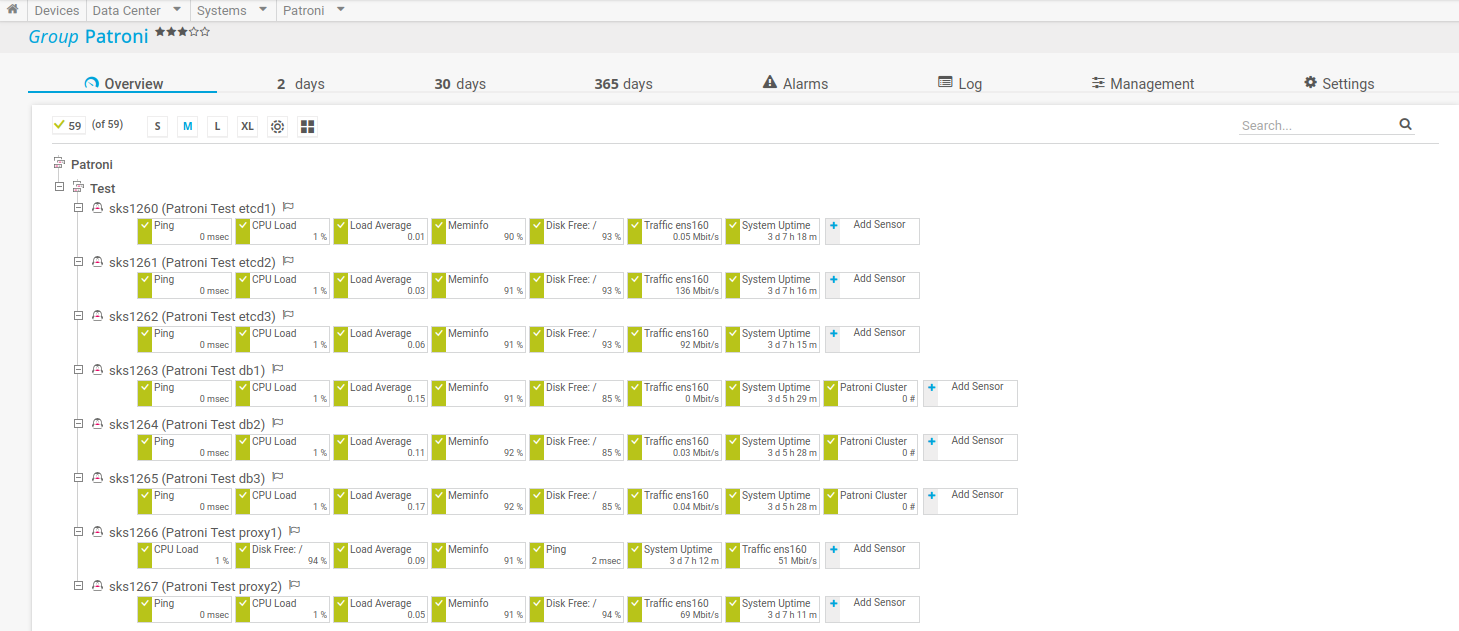
\includegraphics[width=1\linewidth]{source/implementation/construction_implementation/monitoring/prtg_patroni}
        \caption{\Gls{PRTG} - Patroni Monitoring}
        \label{fig:prtg_patroni}
    \end{figure}
\end{flushleft}
\begin{flushleft}
    Zusätzlich wurde ein Python Custom Sensor erstellt.\\
    Dieser nutzt die Patroni REST-API um folgende Werte abzufragen:
    \begin{description}
        \item \textbf{Cluster Status}\hfill \\Prüft, ob der Cluster noch im Status running ist.\\Dabei wird geprüft ob der Cluster \guillemotleft running\guillemotright ist.\\Ist der Cluster pausiert, wird eine Warnung ausgegeben.\\Andernfalls wird ein Fehler geworfen.
        \item \textbf{Cluster Unlock}\hfill \\
        \item \textbf{Failsafe Mode Activity}\hfill \\
        \item \textbf{Replication Lag}\hfill \\
        \item \textbf{Replication State}\hfill \\
    \end{description}


    \begin{figure}[H]
        \centering
        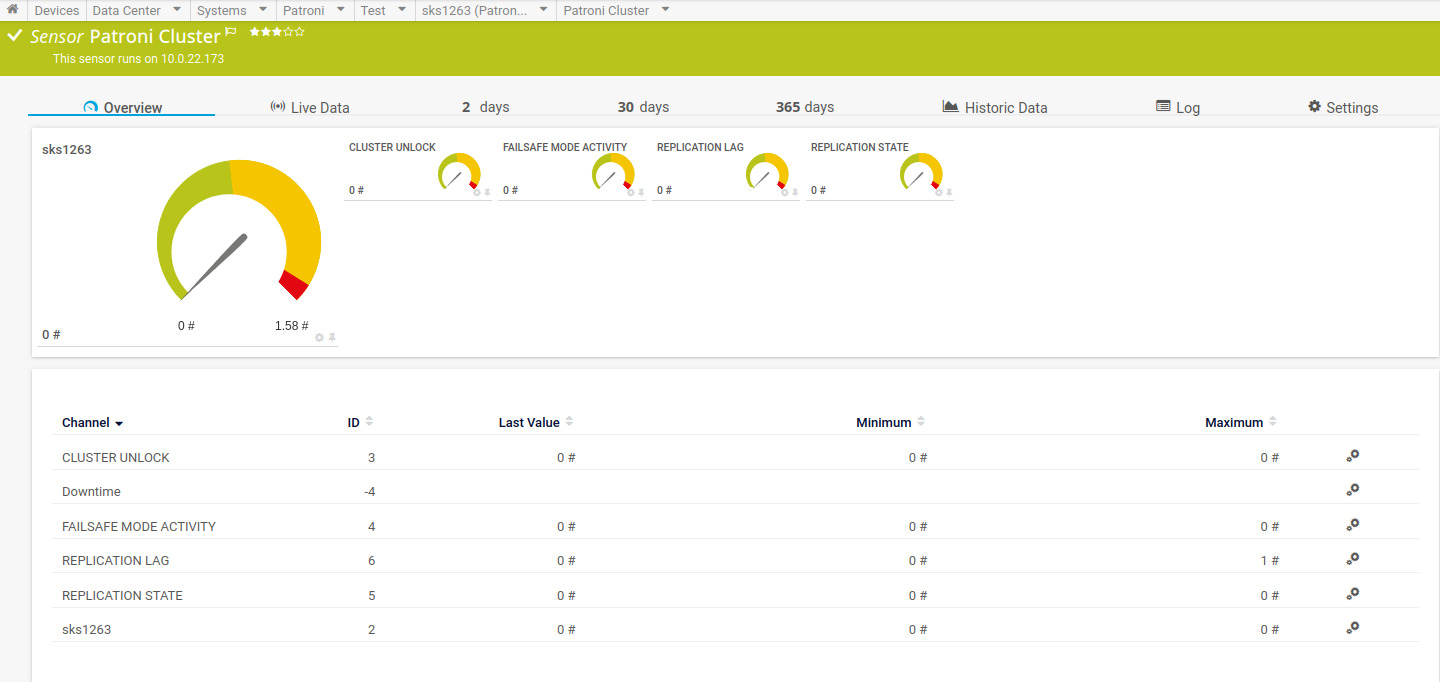
\includegraphics[width=1\linewidth]{source/implementation/construction_implementation/monitoring/patroni_cluster_sensor}
        \caption{\Gls{PRTG} - Patroni Cluster Sensor}
        \label{fig:patroni_cluster_sensor}
    \end{figure}
\end{flushleft}